	\chapter{Modell} \label{chapter: Modell}
	In this paper, the prediction of rental price intervals is investigated using statistical and machine learning methods. In particular, the focus is briefly on the application of linear regression and decision trees. This focus is necessary to obtain a comparative model for a neural network developed later. For this purpose, the data set is divided into training and test data in a ratio of 80:20.  An accuracy dataset is also created documenting the error functions ME (Mean Error), RMSE (Root Mean Squared Error), MAE (Mean Absolute Error), MPE (Mean
	Percentage Error) and MAPE (Mean Absolute Percentage Error). The focus is on the RMSE. In addition, the name of the model and the runtime (in minutes) are added to the data set. The column 'Warm rent' documents whether the Accuracy values refer to warm or cold rent. The column 'Train\_test' documents whether the Accuracy values refer to the training or test data. In addition, 'Seed' is listed to allow the data to be reproduced. The empty data set that is filled with the following models is of the following shape:

	\begin{table}[H]
	\begin{verbatim}
		ME RMSE MAE MPE MAPE                     Name  Zeit Warmmiete train_test seed
		-----------------------------------------------------------------------------
	\end{verbatim}
	\caption{Accuracy table: empty data set}
	\label{tbl: lm-Modell}
\end{table}

	\section{Linear regression} \label{subsec: lineare Regression}
	Linear regression is a simple and widely used statistical model used to explain a dependent variable in terms of one or more independent variables. It assumes that there is a linear relationship between the variables \cite{LM}. In this paper, an attempt is made to predict rental prices based on various characteristics of the apartments, such as size, location and condition of the apartment. To do this, we first develop a linear regression model for warm rent that represents rent prices as a function of characteristics.
	The anova analysis for the first linear model found that the features documents, firing type, and flat rent had no significant effect on the model. After removing these data and running a regression again, the result was the table\ref{tbl: lm-Modell}. This first table suggests that linear regression in this form does not provide good predictions for the test data. The model fits the training data much better than the test data. However, it is not possible to make a final assessment of the model until a comparative model has been constructed.
	
	\begin{table}[H]
		\begin{verbatim}
    ME RMSE MAE MPE MAPE                     Name  Zeit Warmmiete train_test seed
    -----------------------------------------------------------------------------
    20  628 231  -2   16                       Lm   0.0      TRUE      train   NA
   -19 1247 243  -3   16                       Lm   0.0      TRUE       test   NA
    21  619 231  -2   16 Lm   - PM - BevArt - Dok   0.0      TRUE      train   NA
   -19 1234 243  -3   16 Lm   - PM - BevArt - Dok   0.0      TRUE       test   NA	
		\end{verbatim}
	\caption{Accuracy table: lm-Modell}
	\label{tbl: lm-Modell}
	\end{table}
	
	\section{XGBoost} \label{subsec: xg}
	XGBoost (Extreme Gradient Boosting) XGBoost belongs to the class of gradient boosting algorithms and combines several weak models into a strong decision tree. In this work, many small trees with a maximum branch depth of 3 are generated. A single tree is extremely weak. The combination of several trees leads to an extremely efficient and strong model.  (vgl. \cite{Data Science Solutions with Python} p.66 and \cite{XG}	).
	The following code shows how to perform cross-validation using XGBoost. First, the optimal number of trees is evaluated and then the final model is created \footnote{Again the note: The number of pages of this term paper is limited. The focus will be on the neural network, so it is not possible to go into details here.}.	
	
	\begin{verbatim}
		param<-list(
		objective = "reg:linear",
		booster = "gbtree",
		eta=0.05, # should prevent overfitting default 0.3
		gamma=0, # 0 - oo - the larger the more conservative  
		max_depth=3, #default=6  - larger trees -> overfitting + speicer problems
		min_child_weight=1, #default=1
		subsample=1
		)
		xgbcv <- xgb.cv( 
		   params = param, 
		   data = xgtrain, 
		   nrounds = 2000, 
		   nfold = 5, # Equal sized samples
		   showsd = T, 
		   stratified = T, 
		   print_every_n = 40,
		   early_stopping_rounds = 10, # if no further improvement -> abort
		   maximize = F, 
		   base_score = .5,
		   prediction = T)
		xgb_mod <- xgb.train(data = xgtrain, params=param, nrounds = xgbcv$best_iteration,base_score =.5)
	\end{verbatim}

\begin{table}[H]
	\begin{verbatim}
   ME RMSE MAE MPE MAPE                     Name  Zeit Warmmiete train_test seed
   -----------------------------------------------------------------------------
   20  628 231  -2   16                       Lm   0.0      TRUE      train   NA
  -19 1247 243  -3   16                       Lm   0.0      TRUE       test   NA
   21  619 231  -2   16 Lm   - PM - BevArt - Dok   0.0      TRUE      train   NA
  -19 1234 243  -3   16 Lm   - PM - BevArt - Dok   0.0      TRUE       test   NA
  -----------------------------------------------------------------------------
   18  204 118  -1    9                   xg 648   0.6      TRUE      train  123
   14  547 189  -2   13                   xg 648   0.6      TRUE       test  123	
	\end{verbatim}
	\caption{Accuracy table: xg-Modell}
	\label{tbl: xg-Modell}
\end{table}

The Accuracy data were added to the table  \ref{tbl: xg-Modell}. Based on the second model, it is already clear how poor the linear regression model actually is. Moreover, based on the test data, the RMSE of 547 EUR is a good value to compete with the neural network. The model is discussed in more detail in section \ref{sec:NN}.

\section{Neural networks}\label{sec:NN}

Now, the rental prices are studied using neural networks. In particular, the R package 'neuralnet' is used to develop a neural network capable of predicting rental prices based on various characteristics of the apartments. The Rprop+ algorithm is used to train and optimize the neural network. Rprop+ is a further development of the Rprop algorithm used for neural network training. It is a so-called 'on-line' optimizer, meaning that it performs weight adjustments during training, rather than before training as in batch optimizers \cite{Riedmill NN 1993}. The Rprop+ algorithm is based on the fact that the learning rate adjusts independently for each weight. Unlike other optimizers such as gradient descent, which adjusts the learning rate for all weights simultaneously, Rprop adjusts the learning rate for each weight individually. It also uses an 'adaptive' learning rate, which means that the learning rate for each weight is adjusted based on the last change in the weight \cite{Ruder NN rprop+}.
Neural networks have emerged in recent years as powerful tools for predicting target variables. They have the ability to learn complex relationships between inputs and outputs, and are able to model nonlinear relationships between features and rent. For the activation function of the neural network used in this work, the logistic function (also called sigmoid function) \ref{Formel: logistic}  was chosen\footnote{Other functions can also be used. The sigmoid function has the advantage that it is defined on the interval 0-1}.

\begin{align}\label{Formel: logistic}
	\sigma(x) = \frac{1}{1 + e^{-x}}
\end{align} 
Here $x$ is the input of the function and $\sigma(x)$ is the output, which is between 0 and 1. This function has the advantage that it restricts the output of the network to a value between 0 and 1, which is advantageous for predictions of probabilities. The rents are previously scaled to an interval between 0 and 1 using the min-max transformation.

\begin{align}
	X_{norm} = \frac{X - X_{min}}{X_{max} - X_{min}}
\end{align}
Where $X$ is the original value ( e.g. rental price), $X_{min}$ is the smallest value of the training data of a variable, $X_{max}$ is the largest value of the training data of a variable and $X_{norm}$ is the normalized value of the variable. It is important to note that the training and test data were each scaled using the max-min values of the training data. This is necessary so that a single data set can be predicted at the end.

The error function used in this work was the Root Mean Squared Error (RMSE). This error function calculates the root mean squared error between the actual and predicted values. 

A neural network with one layer and one neuron was first created. Surprisingly, already the first neural network gave better results than all models before\footnote{based on the RMSE}, so the run was repeated with a different seed, as shown in Table \ref{tbl: nn-Modell I}. 

\begin{table}[H]
	\begin{verbatim}
   ME RMSE MAE MPE MAPE                     Name  Zeit Warmmiete train_test seed
   -----------------------------------------------------------------------------
   20  628 231  -2   16                       Lm   0.0      TRUE      train   NA
  -19 1247 243  -3   16                       Lm   0.0      TRUE       test   NA
   21  619 231  -2   16 Lm   - PM - BevArt - Dok   0.0      TRUE      train   NA
  -19 1234 243  -3   16 Lm   - PM - BevArt - Dok   0.0      TRUE       test   NA
  -----------------------------------------------------------------------------
   18  204 118  -1    9                   xg 648   0.6      TRUE      train  123
   14  547 189  -2   13                   xg 648   0.6      TRUE       test  123
   -----------------------------------------------------------------------------
   37  481 227  -2   15                  nn c(1)   2.2      TRUE      train    1
   23  423 214  -3   15                  nn c(1)   2.2      TRUE       test    1
   37  483 226  -2   15                  nn c(1)   0.5      TRUE      train    2
   22  397 211  -3   15                  nn c(1)   0.5      TRUE       test    2	
	\end{verbatim}
	\caption{Accuracy table: nn-Modell I}
	\label{tbl: nn-Modell I}
\end{table}

However, it should be noted that one layer and one neuron might not be enough for a more complex problem and it is recommended to add more layers and neurons to improve the performance of the model \cite{Deep Learning Goodfellow}. Therefore, another experiment was performed by creating a layer with two neurons. The results are shown in Table \ref{tbl: nn-Modell II}.

\begin{table}[H]
	\begin{verbatim}
   ME RMSE MAE MPE MAPE                     Name  Zeit Warmmiete train_test seed
   -----------------------------------------------------------------------------
   20  628 231  -2   16                       Lm   0.0      TRUE      train   NA
  -19 1247 243  -3   16                       Lm   0.0      TRUE       test   NA
   21  619 231  -2   16 Lm   - PM - BevArt - Dok   0.0      TRUE      train   NA
  -19 1234 243  -3   16 Lm   - PM - BevArt - Dok   0.0      TRUE       test   NA
  -----------------------------------------------------------------------------
   18  204 118  -1    9                   xg 648   0.6      TRUE      train  123
   14  547 189  -2   13                   xg 648   0.6      TRUE       test  123
   -----------------------------------------------------------------------------
   37  481 227  -2   15                  nn c(1)   2.2      TRUE      train    1
   23  423 214  -3   15                  nn c(1)   2.2      TRUE       test    1
   37  483 226  -2   15                  nn c(1)   0.5      TRUE      train    2
   22  397 211  -3   15                  nn c(1)   0.5      TRUE       test    2
   -----------------------------------------------------------------------------
   35  475 224  -2   15                  nn c(2)   0.4      TRUE      train    1
   20  395 210  -3   15                  nn c(2)   0.4      TRUE       test    1
   32  450 213  -2   15                  nn c(2)   1.0      TRUE      train    2
   15  417 209  -3   15                  nn c(2)   1.0      TRUE       test    2 	
	\end{verbatim}
	\caption{Accuracy table: nn-Modell II}
	\label{tbl: nn-Modell II}
\end{table}

Interestingly, the runtimes do not increase significantly in these first examples. Furthermore, it cannot be clearly determined whether a neural network with two neurons is better than a neural network with one neuron. The results depend on the randomly chosen weights and the other hyperparameters\footnote{The hyperparameters were always identical in order to compare the models. Generally speaking, the result naturally depends on the hyperparameters}. Therefore, in the further course of the experiment, different more complex neural networks are investigated in order to evaluate the performance. For this purpose, the following networks were chosen arbitrarily:

\begin{itemize}
	\item c(4,2) - 2 layers with 4 and 2 neurons 
	\item c(5,3) - 2 layers with  4 and 3 neurons
	\item c(3,2,1) - 3 layers with  3, 2 and one neurons
	\item c(6,3,2) - 3 layers with  6,3 and two neurons
\end{itemize}

\section{Forecast} \label{sec: prediction}

	The table \ref{tbl: nn-Modell III} is interesting from several points of view. On the one hand, it is clear that the running times increase. The neural network with 3 layers and six, three and one neuron ran for 12.6 minutes. The seed data also indicates that it took three runs for the neural network to converge. Thus, the 12 minutes is deceiving, as the first two runs ran longer than 12 minutes without obtaining a valid model. A neural network may not converge for several reasons, such as the initial values of the weights, the number of neurons, the learning rate, and the choice of error function. In this case, the network could not converge because the learning rate was set too high or the number of maximum passes (100,000) was set too low. Thus, the weights could not reach an optimal minimum. It should also be noted that the results (RMSE) did not clearly improve based on the test data. The models clearly depend on the initial values. To deal with this problem, bootstrap aggregation was performed.


\begin{table}[H]	
	\begin{verbatim}
   ME RMSE MAE MPE MAPE                     Name  Zeit Warmmiete train_test seed
   -----------------------------------------------------------------------------
   20  628 231  -2   16                       Lm   0.0      TRUE      train   NA
  -19 1247 243  -3   16                       Lm   0.0      TRUE       test   NA
   21  619 231  -2   16 Lm   - PM - BevArt - Dok   0.0      TRUE      train   NA
  -19 1234 243  -3   16 Lm   - PM - BevArt - Dok   0.0      TRUE       test   NA
  -----------------------------------------------------------------------------
   18  204 118  -1    9                   xg 648   0.6      TRUE      train  123
   14  547 189  -2   13                   xg 648   0.6      TRUE       test  123
  -----------------------------------------------------------------------------
   37  481 227  -2   15                  nn c(1)   2.2      TRUE      train    1
   23  423 214  -3   15                  nn c(1)   2.2      TRUE       test    1
   37  483 226  -2   15                  nn c(1)   0.5      TRUE      train    2
   22  397 211  -3   15                  nn c(1)   0.5      TRUE       test    2
  -----------------------------------------------------------------------------
   35  475 224  -2   15                  nn c(2)   0.4      TRUE      train    1
   20  395 210  -3   15                  nn c(2)   0.4      TRUE       test    1
   32  450 213  -2   15                  nn c(2)   1.0      TRUE      train    2
   15  417 209  -3   15                  nn c(2)   1.0      TRUE       test    2 
  -----------------------------------------------------------------------------
   25  379 189  -2   13                nn c(4,2)   7.7      TRUE      train    1
    1  374 201  -3   15                nn c(4,2)   7.7      TRUE       test    1
   24  397 193  -2   13                nn c(4,2)   6.9      TRUE      train    3
   -1  586 210  -3   15                nn c(4,2)   6.9      TRUE       test    3	
  -----------------------------------------------------------------------------
   22  344 176  -1   13                nn c(5,3)   6.0      TRUE      train    2
   16  485 214  -3   15                nn c(5,3)   6.0      TRUE       test    2
  -----------------------------------------------------------------------------
   28  404 195  -2   14              nn c(3,2,1)   3.0      TRUE      train    3
   11  415 201  -3   15              nn c(3,2,1)   3.0      TRUE       test    3
  -----------------------------------------------------------------------------
   21  346 173  -1   12              nn c(6,3,2)  18.1      TRUE      train    1
    6  399 201  -3   15              nn c(6,3,2)  18.1      TRUE       test    1
   24  380 175  -1   12              nn c(6,3,1)  12.6      TRUE      train    3
   -1  461 217  -3   16              nn c(6,3,1)  12.6      TRUE       test    3
  -----------------------------------------------------------------------------
	\end{verbatim}
	\caption{Accuracy table: nn-Modell III}
	\label{tbl: nn-Modell III}
\end{table}
	
	
	\subsection{Bootstrap Aggregation} \label{subsec: boot}
	Bootstrap aggregation (also called bagging) is a technique used to reduce the uncertainty of estimates by creating random subsets from the original dataset \cite{Bootstrap}. This method creates new datasets by selecting random data with layback from the existing training dataset. The result is a collection of models trained on different data. In this case, bootstrap aggregation was used to reduce the uncertainty of the estimates and improve the results. The training dataset consisted of 5215 records. Thus, 5215 data sets were pulled from the training dataset in each run with layback and six different models were created.


	 \begin{itemize}
	 	\item c(1) one layer and one neuron
	 	\item c(2) one layer and two neurons
	 	\item c(3) one layer and three neurons
	 	\item c(4,1) two layers with 4 and one neuron
	 	\item c(4,2) two layers with 4 and two neurons
	 	\item c(4,3) two layers with 4 and three neurons
	 \end{itemize}
	 
	 For the first three models, 50 runs were selected. However, due to run time, only 20 runs were selected for the last three models. A data matrix with 210 columns and 5215 rows was created. The first 50 columns refer to the first model, the next 50 columns refer to the second model, and so on. When the mean of the first 50 columns is calculated, the result is a more stable prediction for a model with one layer and one neuron. The results for the test data are shown in Table \ref{tbl: bagging}.

	          

\begin{table}[H]
 	\begin{verbatim}
   ME  RMSE   MAE  MPE MAPE   Name Mean.Zeit Warmmiete train_test Durchlaeufe Konvergiert
   --------------------------------------------------------------------------------------
 21.7 406.0 213.0 -2.6 15.5   c(1)       3.4      TRUE       Test          50          50
 18.8 388.0 207.0 -2.7 15.1   c(2)       4.1      TRUE       Test          50          33
 1.9  342.0 190.0 -3.0 14.3   c(3)       8.0      TRUE       Test          50          33
 8.6  379.0 189.0 -3.1 14.0 c(4,1)       9.7      TRUE       Test          20          14
-1.9  363.0 192.0 -3.6 14.4 c(4,2)      14.1      TRUE       Test          20          11
 1.9  340.0 188.0 -3.1 14.2 c(4,3)      12.1      TRUE       Test          20          14
   --------------------------------------------------------------------------------------
 20.8 350.4 190.7 -3.3 17.9   c(1)       3.4     FALSE       Test          50          50
 21.6 345.2 187.2 -3.2 17.6   c(2)       4.1     FALSE       Test          50          33
 2.0  334.3 173.2 -3.7 16.5   c(3)       8.0     FALSE       Test          50          33
 7.8  320.0 168.2 -3.8 16.1 c(4,1)       9.7     FALSE       Test          20          14
-1.3  315.5 170.4 -4.4 16.6 c(4,2)      14.1     FALSE       Test          20          11
 3.5  302.8 168.0 -3.7 16.4 c(4,3)      12.1     FALSE       Test          20          14
    --------------------------------------------------------------------------------------
 	\end{verbatim}
 \caption{Bootstrap Aggregation}
 \label{tbl: bagging}
\end{table}

	It can be seen that the average runtime of a model increases significantly when the number of neurons and layers is increased. Moreover, it can be seen that only the model with one layer and one neuron never had problems with convergence. It converged in 50 out of 50 trials. In percentage terms, more models converged for the more complex models c(4,1) and c(4,3) than for the models with two and three neurons and one layer, respectively. The c(4,2) model had the most difficulty, with only 55 \% converged models. It is also observed that the more complex models with two shifts give better results for cold rent, while this is not necessarily the case for warm rent. One advantage of bagging that has not been mentioned so far is that prediction intervals can now be created. The equation shows the calculation \ref{Formel: VI}.

\begin{align}\label{Formel: VI}
	VI=\vec{\overline{x}} \pm a \cdot \vec{s_x}
\end{align} 

	Where $\vec{s_x}$ is the vector of standard deviations of each data set and $\vec{\overline{x}}$ corresponds to the arithmetic mean of the forecasts. The value $a$ is not clearly defined in the literature and depends on what the prediction is intended to achieve. In this work, the value 1 and 2 were tested first and then it was decided to use 1.5, so that on the one hand the intervals do not become too large and there is enough data in the interval. It was also decided to use only the last 60 models with two layers, on the basis of which the following prediction intervals were calculated.

\subsection{Prediction intervals}

	Based on the formula \ref{Formel: VI} results in some intervals that are relatively small and others that are very large. Relatively precise forecasts could be made for some data, but not for others. Figure \ref{fig: HIST VI} shows an example forecast interval where the actual price of a test data set is not in the forecast interval. In the further course, these are referred to as hits and no hits, respectively.


\begin{figure}[h!]
	\centering
	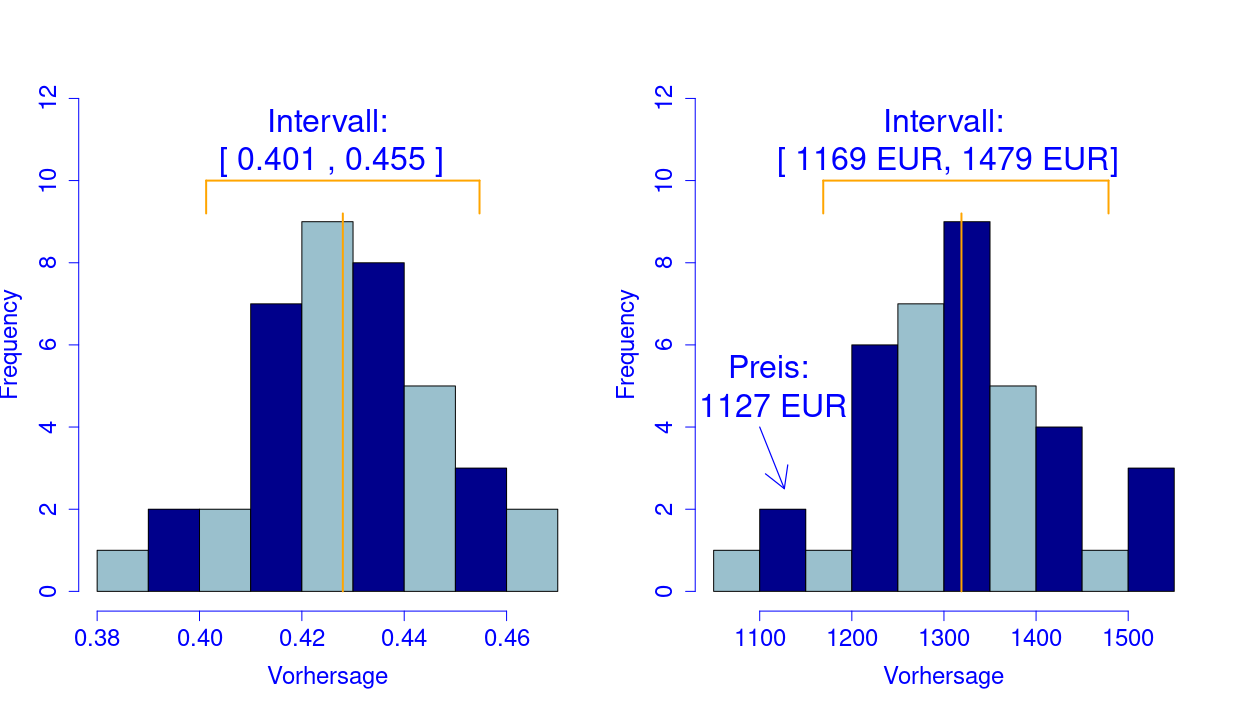
\includegraphics[width=.9\linewidth]{img/hist KI}
	\caption{Prediction interval. Left before the back transformation. Right after the back transformation}
	\label{fig: HIST VI}
\end{figure}

		For the entire test data, this modeling yields the five largest forecast intervals (warm rent) in table\ref{tbl: top 5 absolut}. Surprisingly, only one warm rent was predicted correctly. 

\begin{table}[H]
	\begin{verbatim}
  Tatsächlicher Preis Unteres Intervall Oberes Intervall Treffer Differenz
1               19850             13000            17000   FALSE      4000
2               12450              9300            11000   FALSE      1700
3               11000              7600             8700   FALSE      1100
4                2300              3900             4800   FALSE       900
5                2700              2600             3400    TRUE       800
	\end{verbatim}
\caption{The five absolute biggest differences}
\label{tbl: top 5 absolut}
\end{table}

		For the five smallest absolute forecast intervals, the modeling also yielded only one hit out of five, as shown in Table\ref{tbl: top 5 absolut unten}.

\begin{table}[H]
	\begin{verbatim}
  Tatsächlicher Preis Unteres Intervall Oberes Intervall Treffer Differenz
1              470.00               470              490    TRUE        20
2              550.00               560              580   FALSE        20
3              558.28               510              530   FALSE        20
4              621.00               630              650   FALSE        20
5              629.00               570              590   FALSE        20
	\end{verbatim}
	\caption{The five absolute biggest differences}
	\label{tbl: top 5 absolut unten}
\end{table}

	The five largest and smallest differences in percentage terms are shown in table  \ref{tbl: top 5 relativ} and \ref{tbl: top 5 relativ unten}. The picture looks a little better for the largest percentage intervals. 

\begin{table}[H]
	\begin{verbatim}
  Tatsächlicher Preis Unteres Intervall Oberes Intervall Treffer Prozent
1                1300              1000             1600    TRUE      60
2                 628               690             1100   FALSE      59
3                1150              1000             1500    TRUE      50
4                1325              1000             1500    TRUE      50
5                 700               820             1200   FALSE      46
	\end{verbatim}
	\caption{The five largest differences in percentage terms}
	\label{tbl: top 5 relativ}
\end{table}


\begin{table}[H]
	\begin{verbatim}
  Tatsächlicher Preis Unteres Intervall Oberes Intervall Treffer Prozent
1             1000.75               980             1000   FALSE       2
2             1008.90               960              980   FALSE       2
3              981.15               950              970   FALSE       2
4              925.25               920              940    TRUE       2
5              837.00               900              920   FALSE       2
	\end{verbatim}
	\caption{The five smallest differences in percentage terms}
	\label{tbl: top 5 relativ unten}
\end{table}

 Overall, this analysis yields only 23 \% hits (294). In 40 \% of the data, the price was overestimated. In 37 \% of the data, the warm rent was underestimated. The residuals in Figure  \ref{fig: warmmiete qq}  clearly show that the model had difficulty with very large and very small rents.
 

\begin{figure}[H]
	\centering
	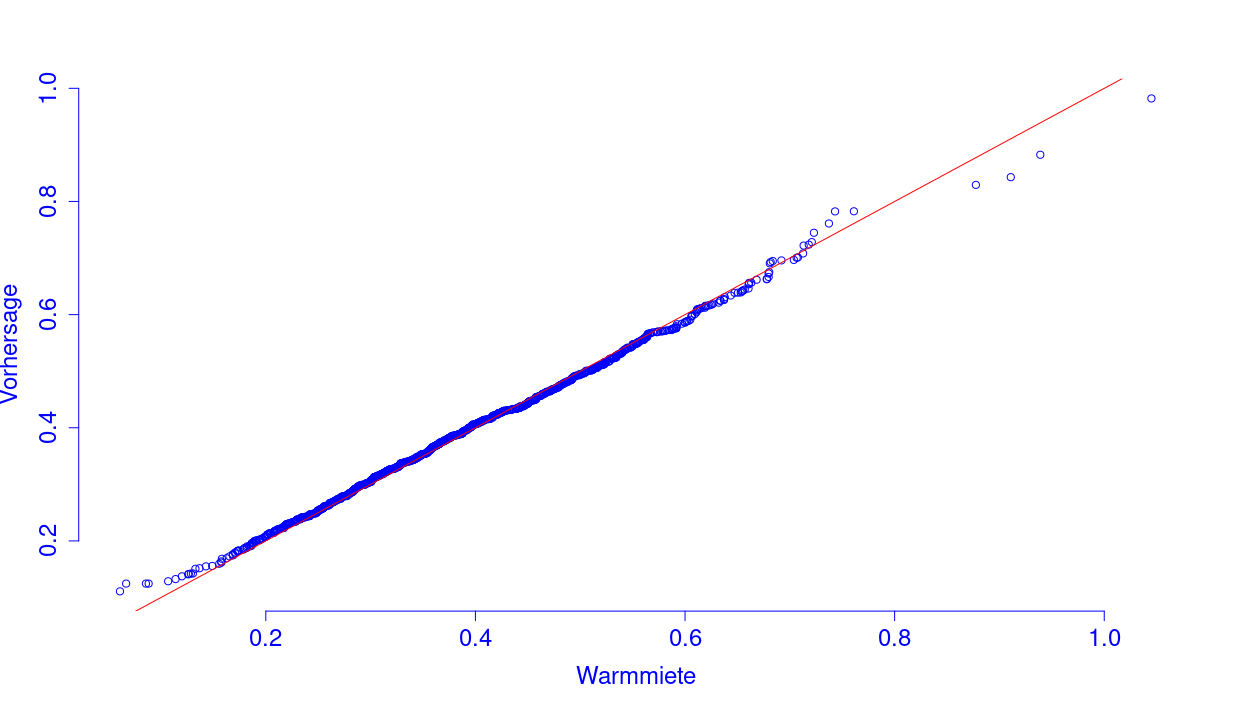
\includegraphics[width=.9\linewidth]{img/warmmiete qq}
	\caption{qqplot cold rent prediction vs. actual value}
	\label{fig: warmmiete qq}
\end{figure}
